% !TeX root = ../main.tex
\chapter{基于高阶全驱系统理论的四旋翼控制器理论设计与数值仿真}  
本章将详细介绍基于高阶全驱系统理论的四旋翼控制器理论设计过程,并开展数值仿真,与经典的四旋翼飞行控制器对比以证明其在控制性能上的优越性。首先,在对比了主要的几种姿态表示方法后,我们选择基于旋转矩阵的姿态表示来建立四旋翼的动力学模型。然后,将欠驱动的四旋翼分解成姿态环路和位置环路,对具有全驱特性的姿态环路应用高阶全驱系统理论,使其从非线性系统转化为线性系统,随即应用LQR控制。最后,在Matlab中展开数值仿真,与经典的SO(3)控制和PX4中的四环PID控制(后简称PID)进行对比。

\section{四旋翼动力学模型和动力分配}
四旋翼的建模可以分成两个部分:一是动力学部分,以作用其上的力和力矩为输入,得到质心加速度和角加速度;二是动力分配部分,以四个电机的控制命令(如pwm占空比)为输入,得到会产生的作用力和力矩。第一部分是理想的物理模型,将四旋翼视作一个刚体,得到普通的刚体动力学模型。第二部分涉及到电机、电调的动态过程,电机转速通过螺旋桨形成推力和反向力矩的过程,以及电池电压对动力套件性能的影响,是实际且工程的,无法用理想的模型去精确地描述。

在理论推导阶段,我们只会用到第一部分的动力学模型,在此之上应用高阶全驱方法设计控制器。而在后续的数值仿真环节中,为了更贴近现实,考虑动力套件的动态过程,我们会这样加入动力分配的环节:将电机转速近似为一阶惯性环节,推力和反向力矩与电机转速的平方近似成正比。

\subsection*{四旋翼动力学模型}
四旋翼在动力学角度可以抽象为一个刚体,和其他任何一个普通的刚体一样。刚体相较于质点,除了质心位置的三个自由度外,还有姿态的三个自由度。刚体的姿态可以由固连在其上的坐标系与地面惯性系之间的线性变换来表示。表示的方式并不唯一,主要包括四元数、轴角、欧拉角和旋转矩阵\cite{attitude}。接下来我们会逐个讨论它们的优劣势。


欧拉角用三次绕轴旋转来描述姿态,这种表示很简洁,只用三个参数即可描述三维旋转,没有冗余。但在数学上,欧拉角存在万向锁问题(Gimbal Lock),在第二个旋转角为$\pm 90^{\circ}$时,第一次旋转和第三次旋转的轴将是相同的,使得三维旋转丢失一个自由度,这被称为奇异性。同时,欧拉角的旋转顺序不可调换,因此旋转顺序在缺乏明确定义的情况下容易引起混淆,欧拉角的导数和机身角速度也只有在小角度条件下才有近似相等的关系,这就给问题的描述带来了不利影响。

由于无法只用三个参数来描述三维旋转而不带奇异性,因此只用四个参数的四元数方法是最紧凑的无奇异性的方式。但四元数在物理意义较明显的问题中,存在运算逻辑不够直观、运算规则较为复杂的缺点。而轴角表示方法虽然有明确的物理意义,便于理解,但是无法直接用于计算。

因此在四旋翼的飞行控制中,学术界最为常用的姿态表示方式是由九个参数构成的旋转矩阵。旋转矩阵$R$是一个行列式为$1$的三维正交矩阵,即$R\in SO(3)$。旋转矩阵的每个列向量  都可以视作是旋转后的每根坐标轴在在原坐标系下的坐标表示,矩阵的各元素也就是两个坐标系基的内积,由于基向量的模为$1$,因此也是各基向量旋转前后夹角的余弦值。故而,旋转矩阵虽然用九个参数来描述旋转有多余的六个约束,但是每个参数都有直观的物理意义,这一点在后续的推导中有很大的优势。此外,虽然$SO(3)$群不是阿贝尔群,但是其对乘法是封闭的,用$R_1R_2^{-1}$就可以很容易地描述$R_1$到$R_2$的旋转。这里我们可以发现,旋转矩阵不仅可以是一个状态量(用以描述姿态),还可以是一个过程量(用以描述旋转),这种形式上的统一是其他描述方式所不具备的。

在选定了刚体姿态表示方式后,接下来需要明确坐标系的定义,机身坐标系$[x_b,y_b,z_b]$ 固连在机身上,如图\ref{fig:1},原点在无人机质心,x轴平行机头方向,z轴竖直向下,y轴定义满足右手定则。世界坐标系$[x_w,y_w,z_w]$则是北-东-地坐标,在室内动捕环境中,东南西北的磁场朝向不再有效,取而代之的是动捕软件中定义的x轴和y轴,这将在后续的章节中展开。
\begin{figure}[!h]
    \centering
    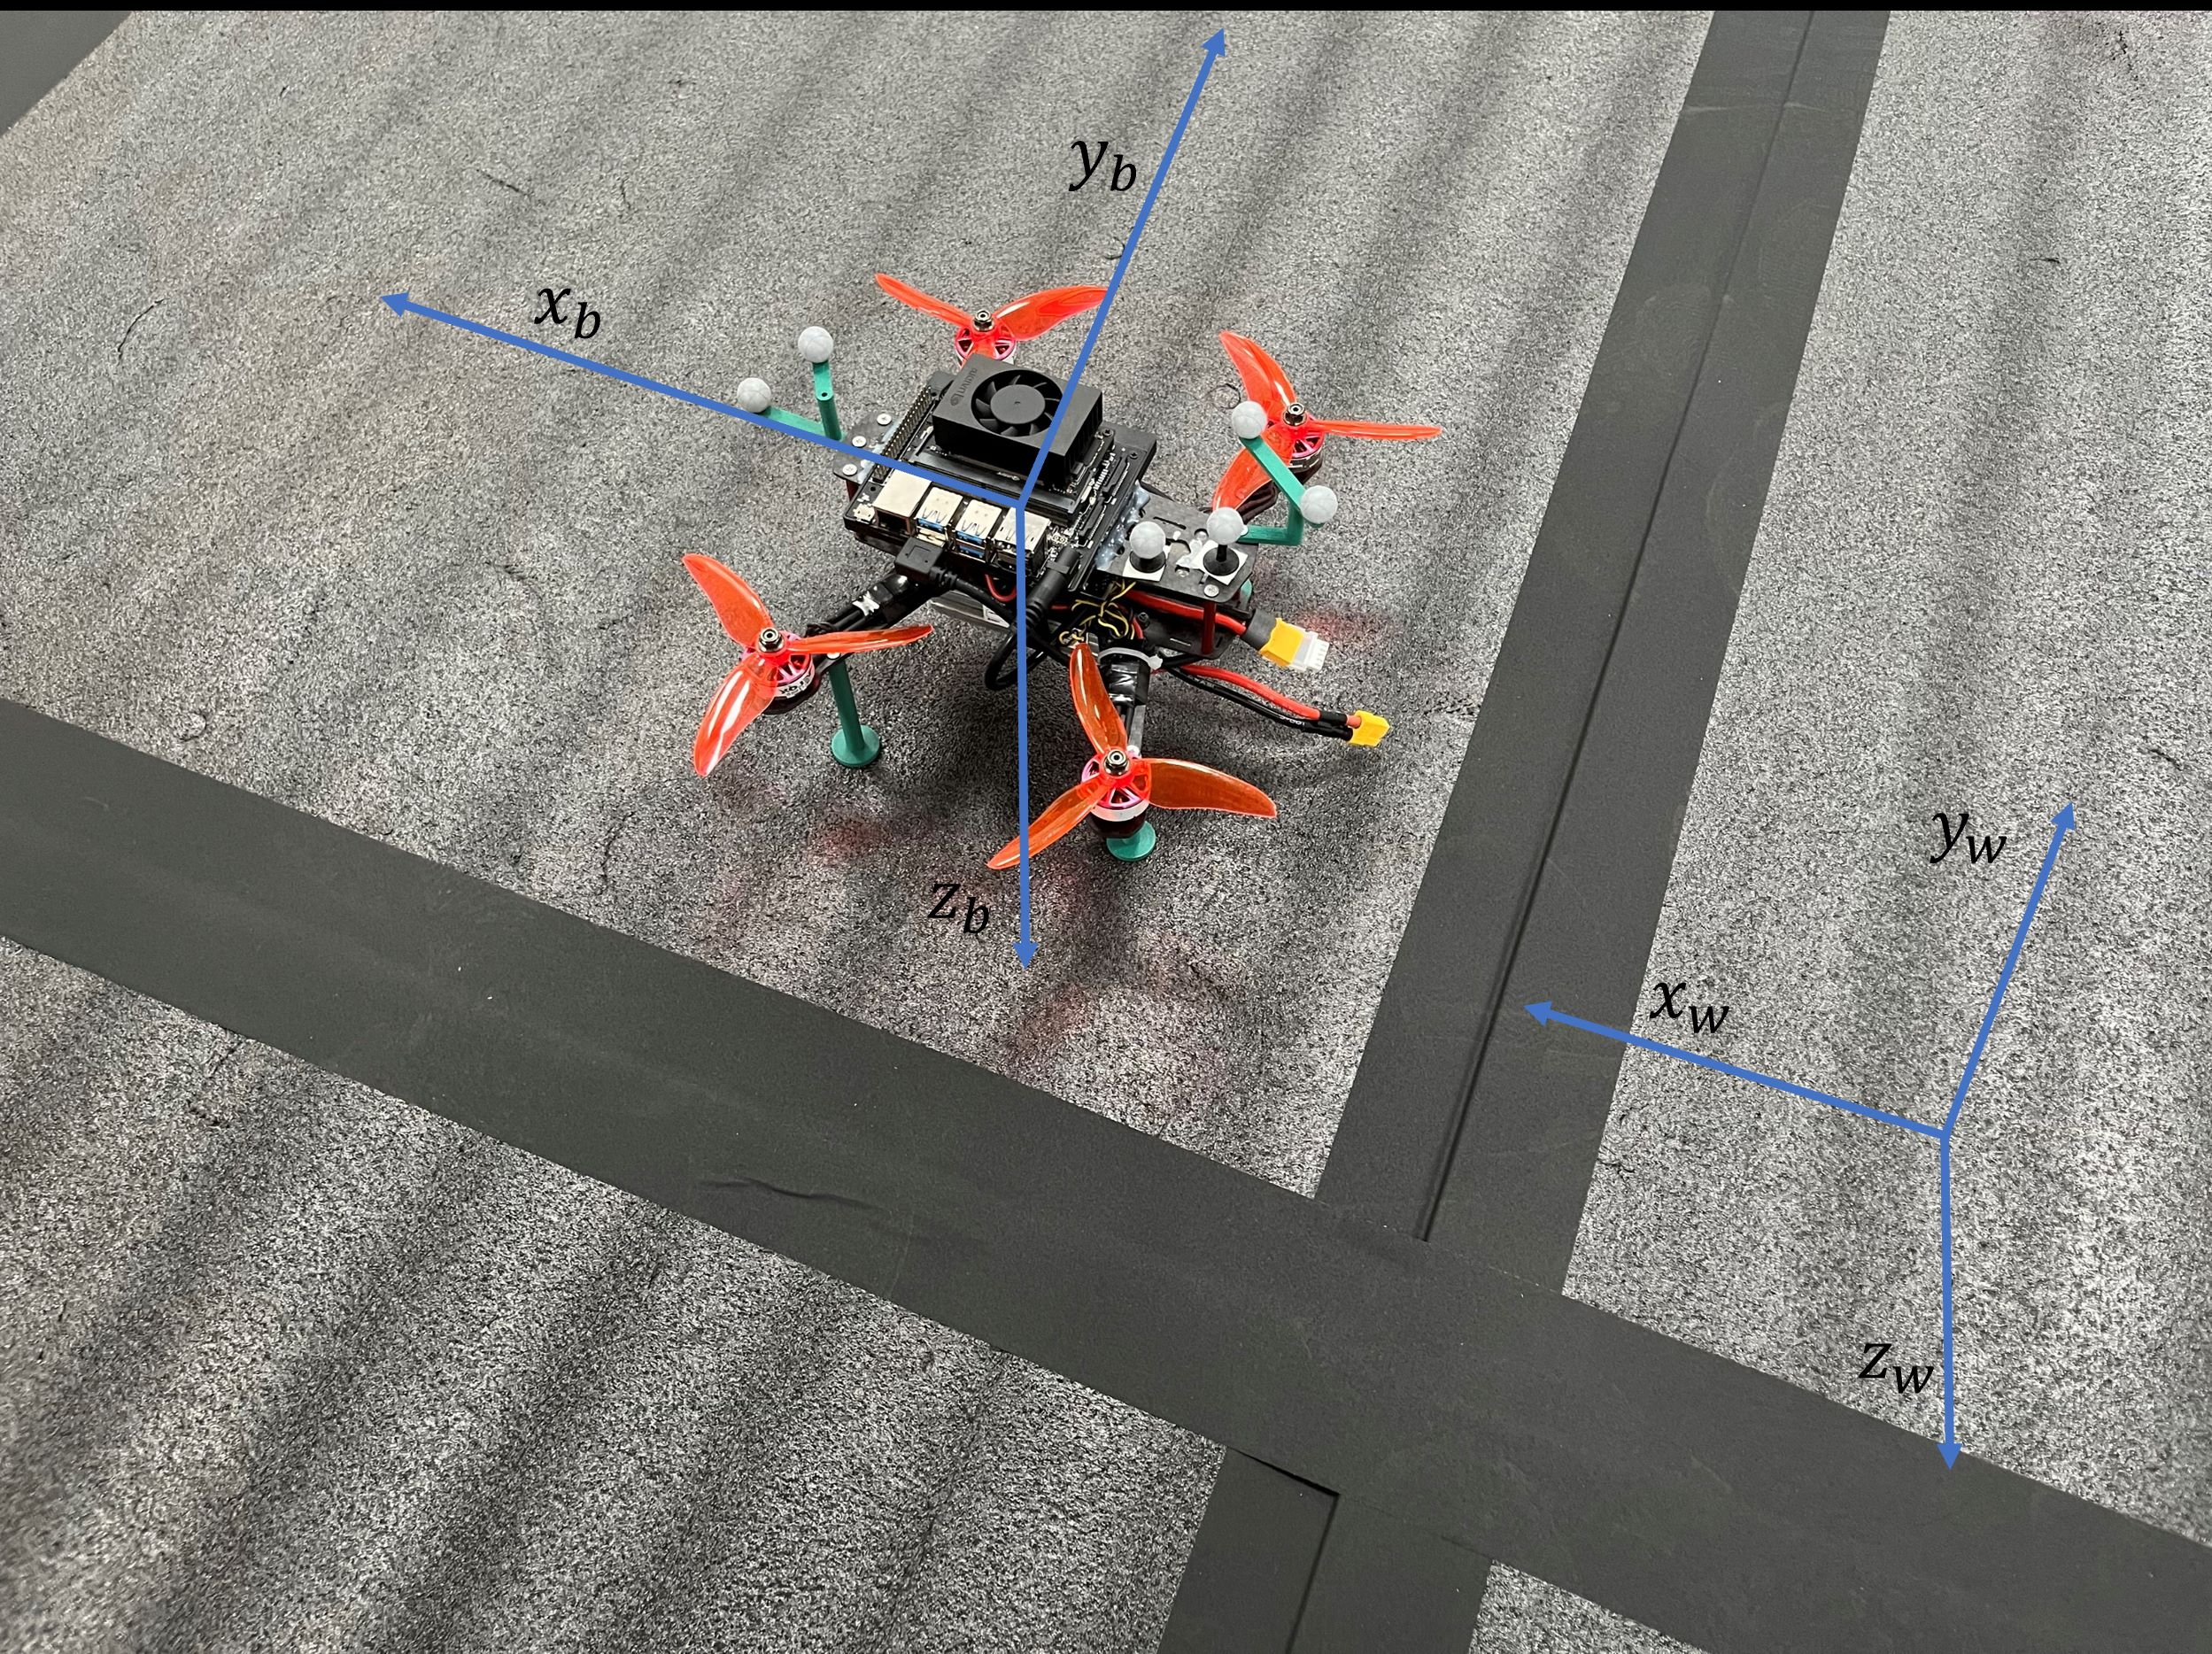
\includegraphics[width=0.7\textwidth]{coordinate.jpg}
    \caption{坐标系定义}
    \label{fig:1}
  \end{figure}

在所有准备工作就绪后,接下来就可以正式进行四旋翼动力学建模。根据牛顿第二定律的质点动力学,由于旋翼的轴都垂直于机身平面,因此在机身坐标系下合力$f$永远是z轴的反方向。
  \begin{equation}
    \dot x=v,
  \end{equation}
  \begin{equation}
    -R \begin{bmatrix} 0\\ 0\\ f \end{bmatrix}+\begin{bmatrix} 0\\ 0\\ mg\end{bmatrix}=m \dot v. 
    \label{equ:a}
  \end{equation}

然后是刚体姿态动力学,为了表示形式的简洁以及工程实际的方便,位置和速度表示在地面系下,而角速度表示在
机身坐标系下,因此刚体动力学方程还要加入补偿的$\omega \times J \omega$项:
  \begin{equation}
    M=J \dot\omega +\omega \times J \omega.
    \label{equ:M}
  \end{equation}

部分文献的建模中加入了电机的陀螺力矩\cite{quanbook},$M_{gyro}=J_{rotor} \omega_{rotor} \times \omega$。 但出于多方面的考虑本文的模型中没有加入这一项:首先,由于控制的分层架构,在工程实现中要实时地得到电机转速并不容易;其次,由叉乘性质可以发现,在电机转矩发生能力较弱的z轴上,陀螺力矩为$0$,其他两个方向上经过估算,与电机能提供的滚转俯仰力矩相比很小,完全可以当作干扰去克服;最后,省略这一项可以方便后面的理论推导。

最后,我们给出旋转矩阵导数和角速度的关系:
  \begin{equation}
    \dot R=R\Omega.
    \label{equ:dotR}
  \end{equation}
推导如下:

设在机身参考系下有一静止的单位向量 $r_0$ ,不妨把 $r_0$ 当作机头的方向向量,它与机体参考系固连,因此不随时间变化,是一个常值。其在世界坐标系下的坐标表示为 $r$,两个坐标表示之间存在关系:
  $$r=R \cdot r_0.$$
等式两边对时间求导,由于 $r_0$ 是常值,可得:
  \begin{equation}
    \dot r= \dot R \cdot r_0.
    \label{equ:1}
  \end{equation}
由于$r$是单位向量长度不变,只考虑世界坐标系中旋转的物理意义,其导数也可以写作:
  \begin{equation}
    \dot r=R \omega \times r.
    \label{equ:2}
  \end{equation}
联立\ref{equ:1}  \ref{equ:2},由叉乘的分配律$A(b\times c)=(Ab)\times (Ac)$可以推出:
$$(R\omega)\times(Rr_0)=\dot R r_0,$$
$$\Rightarrow R(\omega \times r_0)=R\Omega r_0=\dot R r_0.$$
因为$r_0$任意,
$$\Rightarrow \dot R=R \Omega'.$$

\subsection*{四旋翼动力分配模型}
上一节得到了力和力矩与机身加速度和角加速度的关系,这一节将讨论预期电机控制命令与力和力矩之间的关系。计算单个旋翼产生的推力和偏航力矩涉及到复杂的空气动力学,但从结果来看,两者都可以近似与转速平方成正比\cite{minimumsnap},即$f_i=k_F \omega_i^2,M_i=k_M \omega_i^2$。在正常工况的范围内,拟合较好。那么同一个旋翼产生的推力和偏航力矩就是正比关系,可以写作$M_i=c_{\tau f}f_i$。由于桨叶旋转会产生反方向力矩这一特性,如果无人机的四个旋翼全部顺时针旋转,这就会使得无人机在悬停时顺时针自转,并且无法通过控制反方向自转,逆时针同理。因此需要将无人机的桨叶配置成两正两反,对角的为一组,这样就能对消偏航力矩。在实践中,系数$c_{\tau f}$往往会非常小,这会使得控制偏航角变得困难,因有些无人机在设计时会给电机轴与机身垂直方向留出$3\sim5^\circ$的倾角,以便于改变偏航力矩。

在无人机的四个旋翼都竖直向下的情况下,无法产生水平方向的力。因此能产生的作用效果可以仅用四个参数表示:垂直机身向下的总推力和绕三个轴的力矩。四旋翼每个电机产生的升力和作用效果之间的关系可以用式(\ref{equ:trans})来描述,由于旋翼数量与作用效果的维数相同,它们之间的关系是一一映射。
\begin{equation}
  \begin{bmatrix}
    f \\
    M_1 \\
     M_2\\M_3
    \end{bmatrix}=\begin{bmatrix}
    1 &1  & 1 & 1 \\
    0 & -d & 0 & d \\
    d & 0 & -d & 0 \\
    -c_{\tau f} & c_{\tau f} & -c_{\tau f} & c_{\tau f} \\
    \end{bmatrix}\begin{bmatrix}
     f_1\\
    f_2 \\
     f_3\\f_4
    \end{bmatrix}  
    \label{equ:trans}
\end{equation}

通过式(\ref{equ:trans}),从期望作用效果算出每个电机的期望推力后,在matlab数值仿真中,我们可以通过平方正比的关系解出期望转速。将电机转速的动态过程近似为一阶惯性环节,进行开环控制,这主要是为了进行初步的模拟,粗略考虑电机时延的影响。而在PX4的动力分配中,会有基于单个电机最大推力估计的归一化,得到向电机发布的pwm百分比控制指令,还会进一步考虑执行器饱和下动力再分配的情况。由于这不是本课题的研究重点,并且PX4能有效地处理这一环节,因此我们不会深入探讨此环节的内部逻辑。


\section{基于高阶全驱系统理论的控制器设计}

由于四旋翼的推力方向只能向下,因此无法在不倾斜的情况下获得水平方向的推力从而改变水平位置。因此刚体的六个自由度无法同时被控制,使得四旋翼欠驱动。因为输入的维度是4,所以能直接控制的状态维度也是4。虽然四旋翼整体并不满足高阶全驱系统理论的要求,但是姿态环的三个自由度是全驱的,这从式(\ref{equ:M})(\ref{equ:dotR})可以清楚得看到。

四旋翼的控制分为两个环路,位置环和姿态环。由于四旋翼输出的推力总是垂直于机身平面向下,因此要控制位置到达设定点,就需要先旋转姿态,以使推力指向设定点。举例来说,向前飞时,需要机身先向前倾斜获得向前的分力。因此姿态的变化先于位置的变化,在实践中,姿态环的控制频率也远大于位置环。姿态环的动力学方程涉及到更强的非线性,并且姿态环一旦能迅速地达到期望值,位置控制也就水到渠成,因此四旋翼的控制中姿态环的难度和重要性都高于位置环。

\begin{figure}[!h]
    \centering
    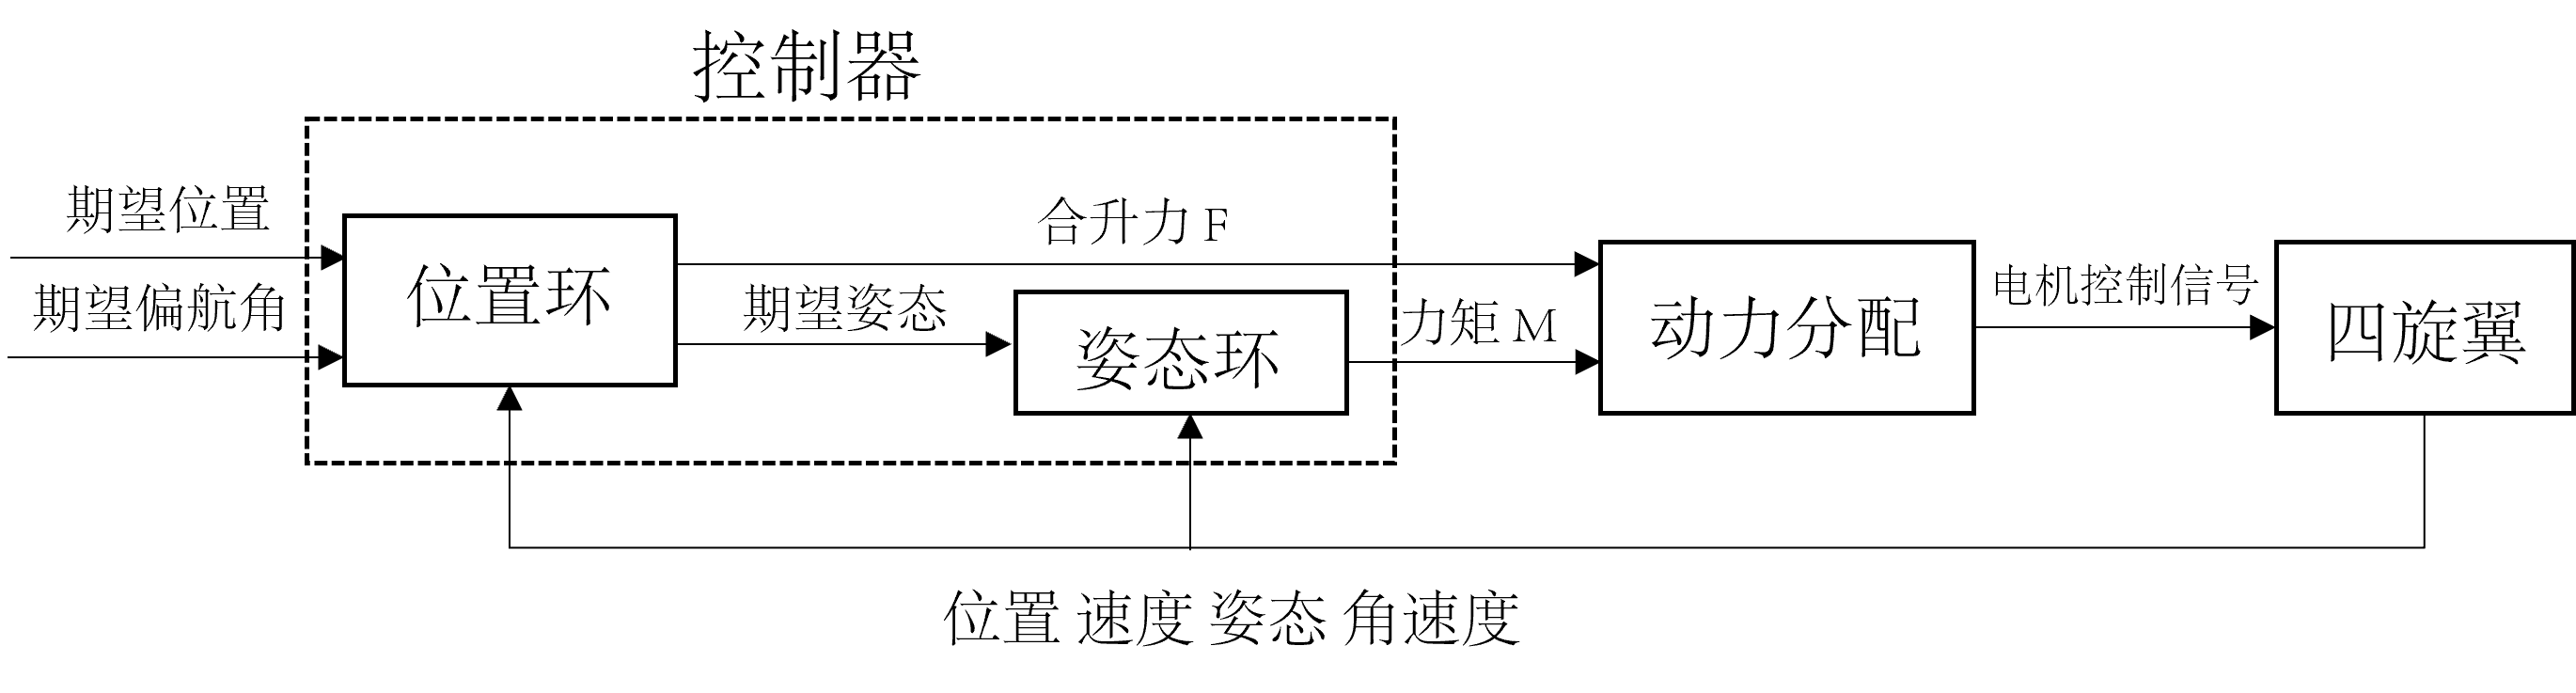
\includegraphics[width=0.7\textwidth]{框图.png}
    \caption{四旋翼控制框图}
    \label{框图}
  \end{figure}
如图\ref{框图},一个典型的四旋翼无人机控制回路会由以下部分组成:
\begin{itemize}
     \item 路径规划,向位置环输入位置设定点
     \item 位置环计算期望推力和期望姿态,将期望姿态发送给姿态环
     \item 姿态环计算期望力矩
     \item 动力分配环节由期望推力和期望力矩计算得到四个电机的控制量
   \end{itemize}

   接下来,我们将分别介绍姿态环路和位置环路的控制器设计。
\subsection*{姿态环路控制器设计}
姿态控制的一大难点就是如何描述当前姿态与期望姿态的误差。由于旋转矩阵所属的$SO(3)$群对加法不封闭,旋转矩阵的差没有物理意义。而且做作差后的三维方阵有九个参数,不满足高阶全驱系统理论的需要。误差需要满足两个条件,一是具有一定的物理意义;二是为使输入矩阵可逆,误差维数要与输入的维数相同,姿态环的输入是三维力矩,因此误差的维数也应当是三。
在这样的要求下,就需要引入轴角表示,接下来介绍旋转矩阵和轴角表示的转换关系。

轴角表示代表了三维旋转最根本的物理含义:任意的三维姿态变换都可以表示为绕某一旋转轴旋转特定角度。在这一思路的指导下,将某个三维向量绕轴旋转到目标向量的旋转矩阵就可以从几何角度这样推导:将该向量分解为平行和垂直旋转轴的两个分量,平行分量对旋转不变,垂直部分的旋转在垂直于转轴的平面内转过目标角度。得到的结果也就是罗德里格斯公式\cite{Rodrigues1840},
\begin{equation}
  R=\cos \theta I+(1- \cos \theta)nn^T+\sin\theta \widehat n,
  \label{equ:Rodrigue}
\end{equation}
其中旋转轴$n \in \mathbb{R}^{3}$,转角$\theta \in \mathbb{R}$。

另外,由于以下两者表述等价:绕轴$n$旋转$\theta$角;以角速度$n$旋转$\theta$时间,旋转矩阵与轴角表示在罗德里格斯公式外还有更简洁的指对映射关系$R=e^{\theta \widehat n}$。推导如下:

对任意$p \in \mathbb{R}^{3}$,其在0时刻的初始值为$p_0$,该向量以角速度$n$旋转,可得:
$$\dot p=n \times p=\widehat n p.$$
求解该微分方程得:
$$p|_{t=\theta}=e^{\theta \widehat n} p_0,$$
即$$\begin{aligned}R=e^{\theta \widehat n}=\sum_{k=0}^\infty \frac{1}{k!}(\theta \widehat n)^k
       =I+\theta \widehat n+\frac{\theta^2}{2 !} \widehat{n}^2+\frac{n^3}{3 !} \widehat{n}^3+\frac{\theta^4}{4 !} \widehat{n}^4\cdots .\end{aligned}      $$
由性质 $(\widehat n)^2=nn^T-I,(\widehat n)^3=-\widehat n$得
$$\begin{aligned}R=e^{\theta \widehat n}&=
      I+\theta \widehat{n}+\frac{\theta^2}{2 !} \widehat{n}^2-\frac{\theta^3}{3 !} \widehat{n}-\frac{\theta^4}{4 !} \widehat{n}^2+\cdots \\
      & =I+\left(\theta-\frac{\theta^3}{3 !}+\frac{\theta^5}{5 !}-\cdots\right) \widehat{n}+\left(\frac{\theta^2}{2 !}-\frac{\theta^4}{4 !}+\frac{\theta^6}{6 !} \cdots\right) \widehat{n}^2 \\
      &=\cos \theta I+(1- \cos \theta)nn^T+\sin\theta \widehat n,
      \end{aligned}      $$
其中$\theta n=\phi \in \mathfrak{so}(3)$是由$SO(3)$李群的切空间得到的李代数\cite{Liegroup}。

从以上旋转矩阵与轴角表示的转换关系可知:
\begin{equation}
  (R-R^T)^\vee=\begin{bmatrix}
    R_{32}-R_{23} \\
    R_{13}-R_{31} \\
    R_{21}-R_{12}
    \end{bmatrix}=2 n \sin\theta.
    \label{error}
\end{equation}
这就是我们所需要的误差表示,维度为三,且具有良好的物理意义。

那么,当前姿态$R$到期望姿态$R_d$的差就可以描述为,
\begin{equation}
    e=(R_d^TR-R^TR_d)^\vee.
\end{equation}
该误差定义不仅可以满足高阶全驱系统理论的要求,并且具有良好的物理意义。当$e\to 0$时,$\theta \to 0$,$R$与$R_d$重合,达到期望。举例来说,当$R$到$R_d$的旋转主要是绕x轴时,那么转轴$n$的x分量也将较大,这就会使得误差的x轴分量最大,也就能根据误差进行状态反馈控制。

在误差定义明确后,接下来根据高阶全驱系统理论的要求,需要对误差连续两次求导,使得方程中出现控制输入,也就是力矩$M$。
$$\begin{aligned}
    \dot e=&[(R_d^TR \Omega-\Omega_dR_d^TR)-(R_d^TR \Omega-\Omega_dR_d^TR)^T]^\vee\\
    =&[R_d^TR(\Omega-R^TR_d \Omega_dR_d^TR)-(R_d^TR(\Omega-R^TR_d \Omega_dR_d^TR))^T]^\vee \\
    =&[R' \hat e_\Omega  + \hat e_\Omega R'^T]^\vee,
\end{aligned} $$
为表达的简洁,定义
    $$R'=R_d^TR, \quad e_\Omega=\omega -R^TR_d \omega_d.$$
进一步求二阶导:
    $$\begin{aligned}
        \ddot e =& [(R' \hat e_\Omega \Omega + R'\dot \Omega -\Omega_d R' \hat e_\Omega -\dot \Omega_d R')-(R' \hat e_\Omega \Omega + R'\dot \Omega -\Omega_d R' \hat e_\Omega -\dot \Omega_d R')^T]^\vee\\
        =&[(R' \hat e_\Omega \Omega  -\Omega_d R' \hat e_\Omega -\dot \Omega_d R')-(R' \hat e_\Omega \Omega  -\Omega_d R' \hat e_\Omega -\dot \Omega_d R')^T]^\vee+[R'\dot \Omega-(R'\dot \Omega)^T]^\vee\\
        =&[(R' \hat e_\Omega \Omega  -\Omega_d R' \hat e_\Omega -\dot \Omega_d R')-(R' \hat e_\Omega \Omega  -\Omega_d R' \hat e_\Omega -\dot \Omega_d R')^T]^\vee\\
        & + \begin{Bmatrix}
        \begin{bmatrix}
        R'_{11} &R'_{12}  & R'_{13} \\
        R'_{21} & R'_{22} & R'_{23} \\
        R'_{31} & R'_{32} &R'_{33}  \\
        \end{bmatrix}&\begin{bmatrix}
        0 & -\dot\omega_3 &\dot\omega_2  \\
         \dot\omega_3& 0 &  -\dot\omega_1\\
         -\dot\omega_2&\dot\omega_1  & 0 \\
        \end{bmatrix}\end{Bmatrix}^\vee -\begin{Bmatrix}
        \begin{bmatrix}
        R'_{11} &R'_{12}  & R'_{13} \\
        R'_{21} & R'_{22} & R'_{23} \\
        R'_{31} & R'_{32} &R'_{33}  \\
        \end{bmatrix}&\begin{bmatrix}
        0 & -\dot\omega_3 &\dot\omega_2  \\
         \dot\omega_3& 0 &  -\dot\omega_1\\
         -\dot\omega_2&\dot\omega_1  & 0 \\
        \end{bmatrix}\end{Bmatrix}^{T\vee}\\
        =&[(R' \hat e_\Omega \Omega  -\Omega_d R' \hat e_\Omega -\dot \Omega_d R')-(R' \hat e_\Omega \Omega  -\Omega_d R' \hat e_\Omega -\dot \Omega_d R')^T]^\vee \\
        & +        \begin{bmatrix}
        R'_{22}+R'_{33} & -R'_{21} & -R'_{31} \\
         -R'_{12}& R'_{11}+R'_{33} & -R'_{32} \\
         -R'_{13}&- R'_{23} & R'_{11}+R'_{22} \\
        \end{bmatrix}\dot \omega\\
        =&A_d+R_B\dot \omega,
        \end{aligned}  $$
其中$$A_d=[(R' \hat e_\Omega \Omega  -\Omega_d R' \hat e_\Omega -\dot \Omega_d R')-(R' \hat e_\Omega \Omega  -\Omega_d R' \hat e_\Omega -\dot \Omega_d R')^T]^\vee,$$

        $$R_B=\begin{bmatrix}
            R'_{22}+R'_{33} & -R'_{21} & -R'_{31} \\
             -R'_{12}& R'_{11}+R'_{33} & -R'_{32} \\
             -R'_{13}&- R'_{23} & R'_{11}+R'_{22} \\
            \end{bmatrix}.$$
代入\ref{equ:M},得:
$$\begin{aligned}
        \ddot e=&A_d+R_B J^{-1}(-\omega \times J\omega+M)\\
        =&A_d-B \omega\times J\omega +BM
        \end{aligned},$$
其中$$B=R_BJ^{-1}.$$
当$B$满秩时,符合全驱条件,可以设计控制律
$$M=-B^{-1} A_d+\omega \times J\omega +B^{-1}M^*,$$
使得原非线性系统转化为线性系统
    $$\ddot e=M^*.$$

 对于该补偿掉所有非线性部分的二阶积分器模型,得到状态空间表示下的方程
    $$\dot x_\omega=\begin{bmatrix}
        0_{3\times 3} & I_{3\times 3} \\
        0_{3\times 3} & 0_{3\times 3}
    \end{bmatrix} x_\omega+\begin{bmatrix}
        0_{3\times 3} \\ I_{3\times 3}
    \end{bmatrix} M^* ,$$
    $$x_\omega=\begin{bmatrix}
        e \\ \dot e.
    \end{bmatrix}$$
在此基础上可以便利地采用任何线性系统控制器设计方法,采用LQR控制器,得到$M^*=-kx_\omega$。那么全部的控制律就是
   $$ \begin{aligned}
        M=&-J R_B^{-1} [(R' \hat e_\Omega \Omega  -\Omega_d R' \hat e_\Omega -\dot \Omega_d R')-(R' \hat e_\Omega \Omega  -\Omega_d R' \hat e_\Omega -\dot \Omega_d R')^T]^\vee \\
         &+\omega \times J\omega + J R_B^{-1}(-kx_\omega).
    \end{aligned}$$

    若$R_B$不满秩,上述高阶全驱方法则不成立。但是不满秩的点在$\mathbb{R^{3 \times 3}}$是无处稠密的,因此在实验中不会遇到。但是为了理论的完备,设置替补控制律\cite{Lee2010}
    $$M=-k_R e_R-k_\omega e_\omega+\omega \times J \omega -J(\Omega R'^T \omega_d-R'^T \dot \omega_d) $$
    $$ e_R=\frac{1}{2} (R'-R'^T)^\vee ,$$
    这种控制律能保证指数收敛,参数$k_R,k_\omega$需要根据转动惯量调试后选定。
    \subsection*{位置环路控制器设计}
    在设计位置环的控制算法时,首先要结合期望偏航角生成期望姿态$R_d$作为姿态环的输入。然后,考虑到姿态环的高响应速度,其动态过程可以被忽略。这一假设进一步简化了位置环的动力学方程,使其也能被视作一个线性系统,仍然先采用LQR方法进行控制。

    期望姿态$R_d$是由位置环输出以及期望偏航角生成的,它代表了要达到期望的位置所需的推力方向。由于无人机的推力只能垂直于机身平面,要到达期望的位置需要有指向该位置的力,因此要首先改变无人机姿态使其法线方向平行于期望推力方向,再结合外部输入的期望偏航角,就能得出期望的姿态\cite{Lee2010}。

    在本课题中,机头的指向即偏航角的重要性相对期望位置较弱,且在姿态较大时,偏航角的意义实质上并不明确:偏航角如果是Z-Y-X欧拉角定义下的第一个转角,当后两个转角较大时,偏航角也就脱离了原本的物理意义。因此首先保证期望推力方向,将其设计成反馈加前馈的形式,
    $$f_{ideal}=k_x e_x+k_v e_v-mg \vec e_3+m a_d,$$
    $$\vec b_{3d}=-\frac{f_{ideal}}{||f_{ideal}||},$$
    $$ e_x=x_d-x ,\quad e_v=v_d-v ,\quad \vec e_3=\begin{matrix}
        [0 & 0 & 1].
    \end{matrix}^T$$
    然后将期望偏航角产生的单位向量$\begin{matrix} [\cos{\psi_d} & \sin{\psi_d} & 0]  \end{matrix}^T$投影到垂直于$b_{3d}$的平面上,就能得到期望姿态$R_d= \begin{matrix} [ \vec b_{2d}\times \vec b_{3d} &\vec b_{2d} & \vec b_{3d}] \end{matrix}$,$\vec b_{2d}=\vec b_{3d} \times \vec b_{1d}$,如图 \ref{fig:2}。
    \begin{figure}[!h]
        \centering
        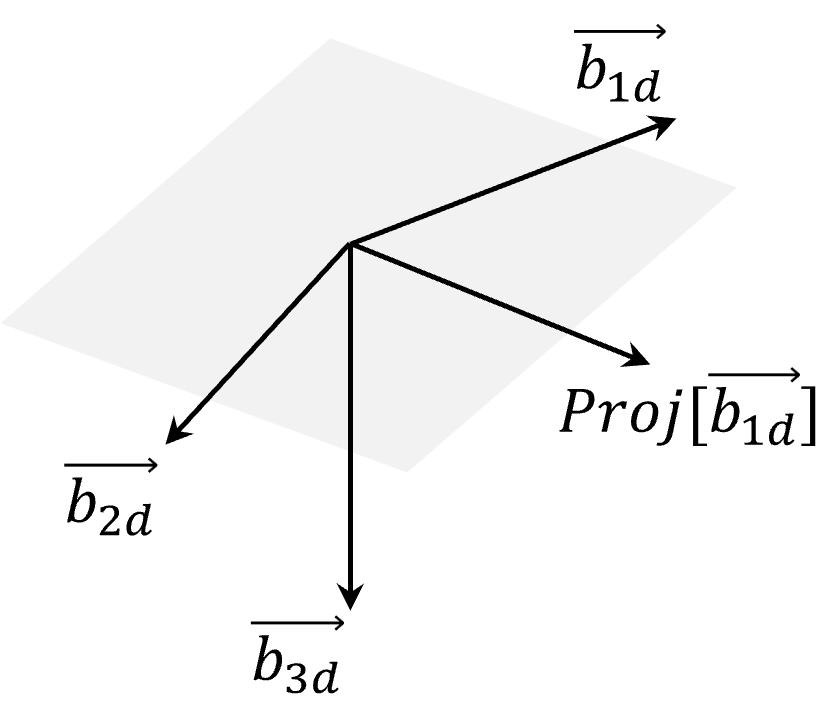
\includegraphics[width=0.3\textwidth]{desired R.png}
        \caption{期望姿态定义}
        \label{fig:2}
      \end{figure}

      以上计算得到的$f_{ideal}$没有考虑姿态动态过程,由于$R$无法瞬间收敛到$R_d$,当姿态尚未收敛时,推力的控制指令应当为$f_{ideal}$在当前姿态推力方向上的投影,
      $$f=f_{ideal}\cdot R e_3,$$否则会在错误的方向上投入过多的力分量。接下来需要得出控制律$k_x , k_v$,当姿态$R$能迅速收敛到$R_d$时,动力学方程(\ref{equ:a})退化为
      $$m \dot v=mge_3-f.$$
      那么位置控制环节就变成了简单的线性系统,可以写作六阶状态空间表示:
      $$\dot x_p=\begin{bmatrix}
        0_{3\times 3} & I_{3\times 3} \\
        0_{3\times 3} & 0_{3\times 3}
    \end{bmatrix} x_p+\begin{bmatrix}
        0_{3\times 3} \\ \frac{1}{m} I_{3\times 3}
    \end{bmatrix} f +\begin{bmatrix}
        0_{3 \times 1} \\ a_d-g \vec e_3 
    \end{bmatrix},$$
    $$x_p=\begin{bmatrix}
        x_d -x \\ v_d -v
    \end{bmatrix}.$$

将$f$写作补偿掉前馈的形式:$f=f^*-mg \vec e_3 +m a_d$。接下来就可以运用LQR方法得到控制律$f^*=-kx$。

\section{数值仿真实验设计}
在控制器理论设计完成后,我们将在Matlab中进行数值仿真实验。Matlab中基于s-function和simulink的仿真,主要是为了在理论层面验证控制算法的性能。在这一章中,我们将与经典的SO(3)控制和PX4中的四环PID控制(后简称PID)对比,说明HOFA方法的优越性。我们在Simulink环境下构建了一个综合仿真模型,该模型不仅包含了刚体动力学和电机动态,还通过s-function实现了姿态环和位置环分离的双环控制器设计。这种设计使得后续的数据分析和研究工作能够更为便捷、高效。

输入信号在控制理论传统的阶跃和斜坡信号之外,为了能直观且综合地体现跟踪性能,我们设计了一个“8”字形轨迹
$$x_d = \begin{matrix}[5\sin(\frac{t}{2}), & 5\cos(\frac{t}{2})\sin(\frac{t}{2}), &-0.1t]\end{matrix}
\quad
\psi_d=0.01t,$$
如图\ref{fig:8}所示。为了全面体现控制算法的跟踪性能,我们并没有对轨迹做特殊的平滑处理,轨迹的导数存在间断点使得高阶导数无穷大,这可以考验无人机在现实中的抗扰性能。为了模拟起飞和悬停,第一秒内轨迹保持在原点不动,否则仿真就会等同在空中释放电机无转速的无人机。
\begin{figure}[!h]
  \centering
  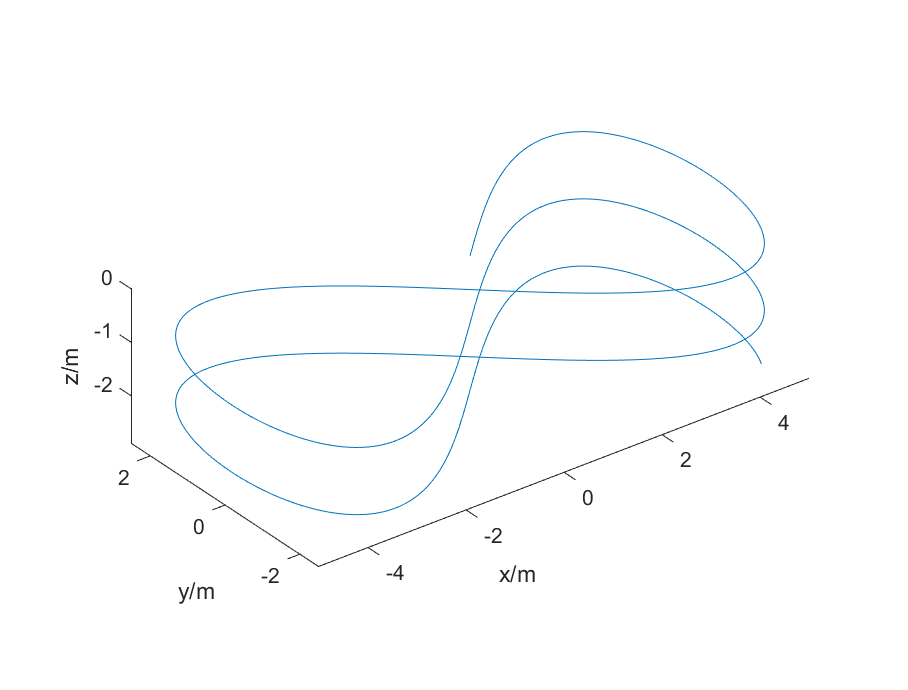
\includegraphics[width=0.5\textwidth]{88.eps}
  \caption{高度匀速上升的“8”字形轨迹(北-东-地坐标系下,地面以上Z轴为负数)}
  \label{fig:8}
\end{figure}

被控对象的建模方面,无人机的刚体动力学部分由simulink中自带的“6DOF block”解决,避免了$SO(3)$群差分近似后单位化的困难。该模块会对外部输入的力和力矩做出反应,返回所需的速度、位置、姿态、角速度等信息。
电机部分,转速的动态由一阶惯性环节表示,根据所选电机型号时间常数$\tau=0.01s$。
姿态控制器和位置控制器分开由两个s-function实现,重力由单独的模块输入到“6DOF block”,如图\ref{fig:sim}所示。
\begin{figure}[!h]
    \centering
    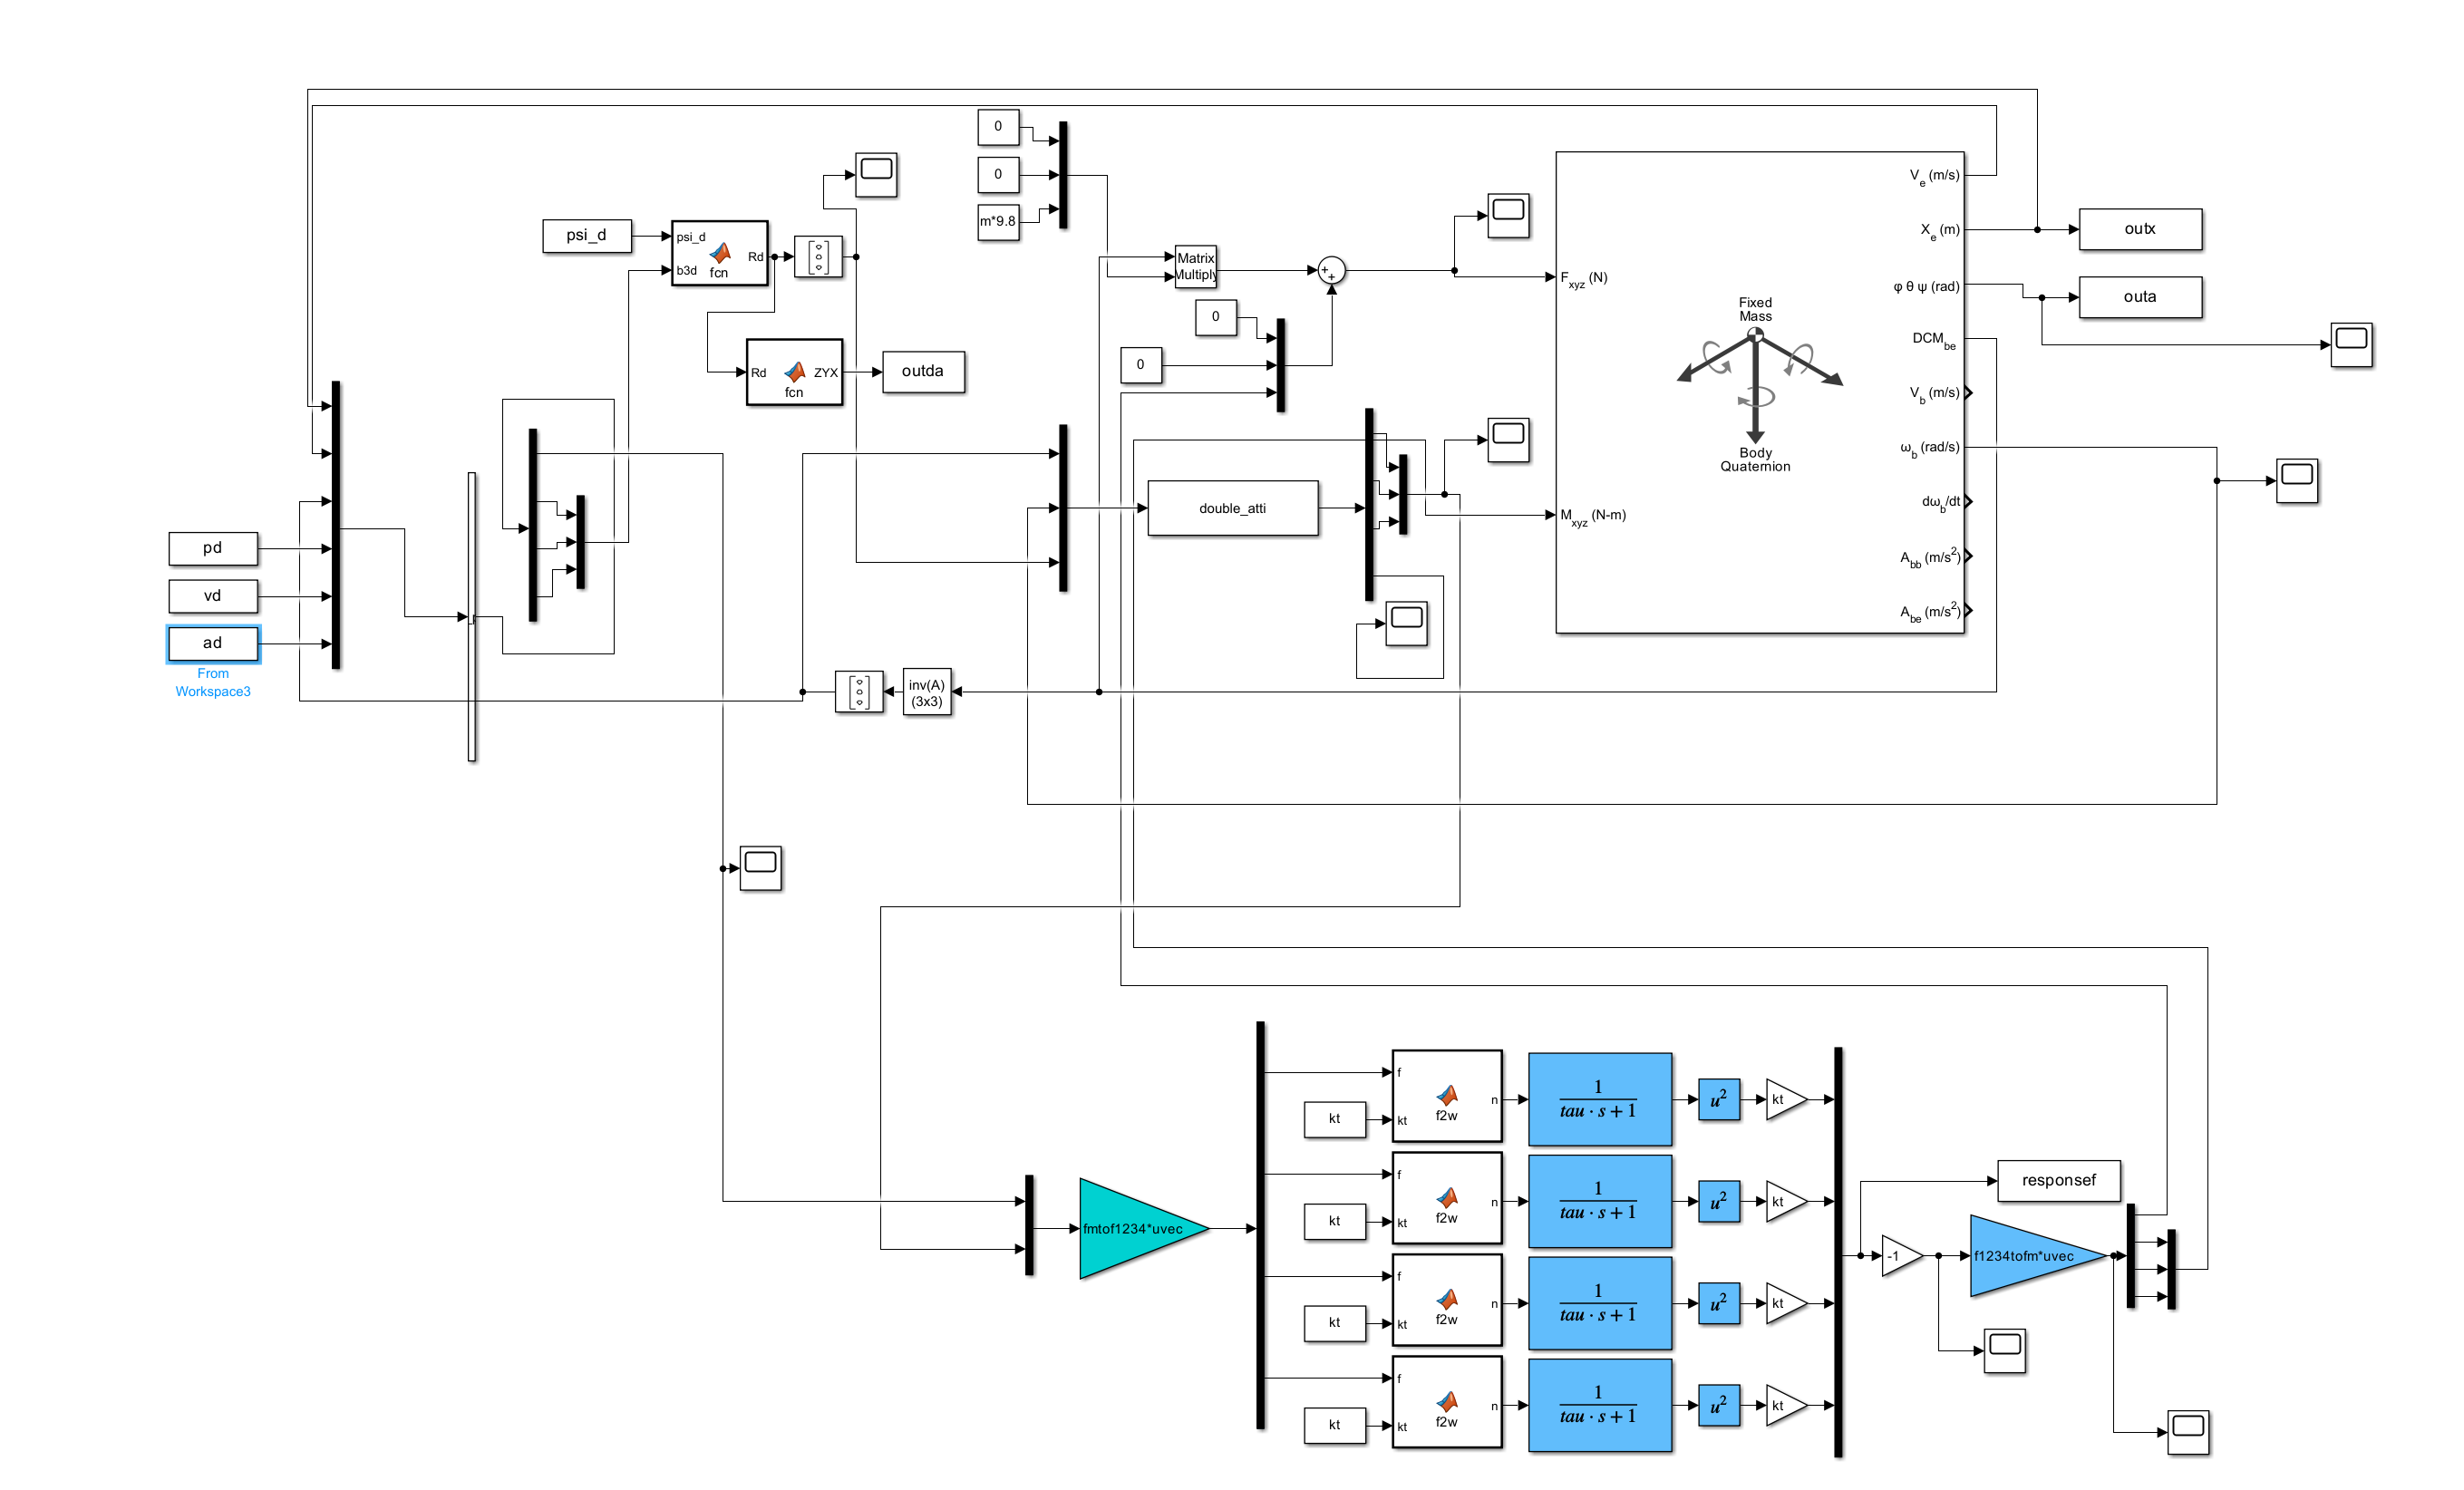
\includegraphics[width=0.9\textwidth]{sim.png}
    \caption{simulink仿真连线图}
    \label{fig:sim}
  \end{figure}

模型参数方面,质量参数由最终实飞的无人机测量得到(见实机实验一章),
$$m=0.8771kg \quad d=0.125m \quad J=\begin{bmatrix}
  0.0031   &      0  &       0\\
  0 &   0.0032      &   0\\
  0  &       0   & 0.0045
\end{bmatrix}kg m^2,$$
电机参数由厂家数据得到,
$$k_t=2.03\times 10^{-8} ,\quad 
\tau=0.01s, \quad
c_{\tau f}=8\times 10^{-3}.$$

控制器参数方面,位置环和姿态环的LQR权重矩阵分别为:
$$Q_x=\begin{bmatrix}
  10&0&0&0&0&0\\
  0&10&0&0&0&0\\
  0&0&10&0&0&0\\
  0&0&0&3&0&0\\
  0&0&0&0&3&0\\
  0&0&0&0&0&3\\
\end{bmatrix}, \quad R_x=\begin{bmatrix}
  0.1 &0 &0\\
  0 &0.1 &0\\
  0 &0 &0.1\\
\end{bmatrix},$$

$$Q=\begin{bmatrix}
  100&0&0&0&0&0\\
  0&100&0&0&0&0\\
  0&0&30&0&0&0\\
  0&0&0&0.1&0&0\\
  0&0&0&0&0.1&0\\
  0&0&0&0&0&0.1\\
\end{bmatrix}, \quad R=\begin{bmatrix}
  0.01 &0 &0\\
  0 &0.01 &0\\
  0 &0 &0.01\\
\end{bmatrix},$$
选择替补姿态控制律
$$k_R=0.881 ,\quad k_\omega=0.254.$$

四旋翼的初始位姿为
$$x(0)=[0,0,0],\quad v(0)=[0,0,0],$$
$$R(0)=I , \quad \omega(0)=[0,0,0].$$

另外,模型还需要做一些工程上的调整。期望值的传递链路是$x_d \to v_d \to R_d \to \omega_d \to \alpha_d$。在这条链路中,除了$ v_d \to R_d$的传递,其他三次都会带来微分,会放大上一环节的噪声。如果放任冲击信号进入控制器,会对系统造成不良影响,因此需要做相应的限幅。但因为期望拉力最大不过接近水平,所以$R_d$这一环节本身就带有限幅,在Matlab仿真中就不做额外限幅以获得更激进的控制效果,同时也能更好地测试姿态环的鲁棒性。

\section{实验结果与分析}

  在实验设计完成后,按照上述参数,在Matlab中用0.005s的控制周期分别运行HOFA、PID和SO(3)控制。输入典型的阶跃和斜坡信号对比其控制性能,由于俯仰与滚转对称,仅选择俯仰模态(x轴)进行实验。

\subsection*{单位阶跃输入}

  在$t=1s$时对x轴输入单位阶跃信号,对比x轴位置、速度、角度、角速度和期望扭矩,如图\ref{matlab_阶跃}。由于另外两轴仅受到轻微的耦合影响,且不是研究对象,为精简篇幅,不在此罗列另外两轴的数据。
\newpage
\newpage
\begin{figure}[!htp]
  \centering
  \begin{subfigure}[t]{0.49\textwidth}
    \centering
    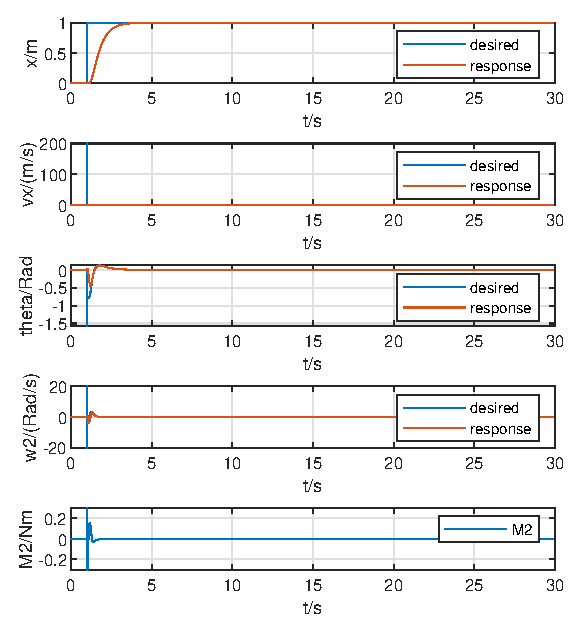
\includegraphics[width=\linewidth]{hofa_1.eps}
    \caption{HOFA}
  \end{subfigure}\hfill
  \begin{subfigure}[t]{0.49\textwidth}
    \centering
    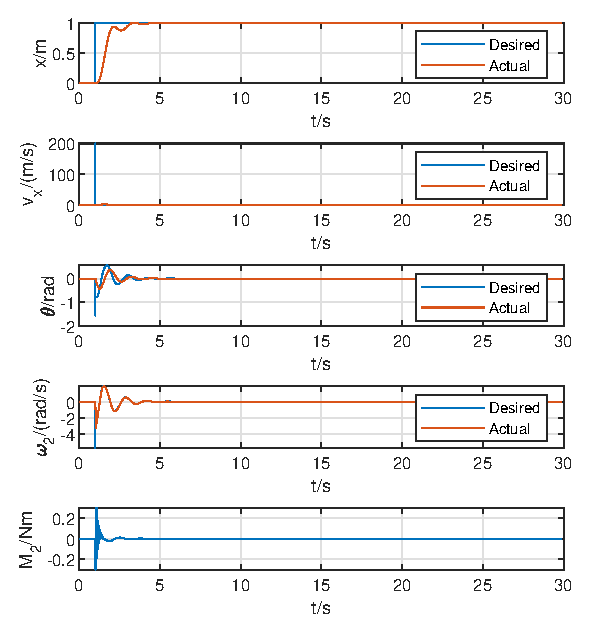
\includegraphics[width=\linewidth]{px4_1.eps}
    \caption{PID}
  \end{subfigure}\hfill
  \begin{subfigure}[t]{0.49\textwidth}
    \centering
    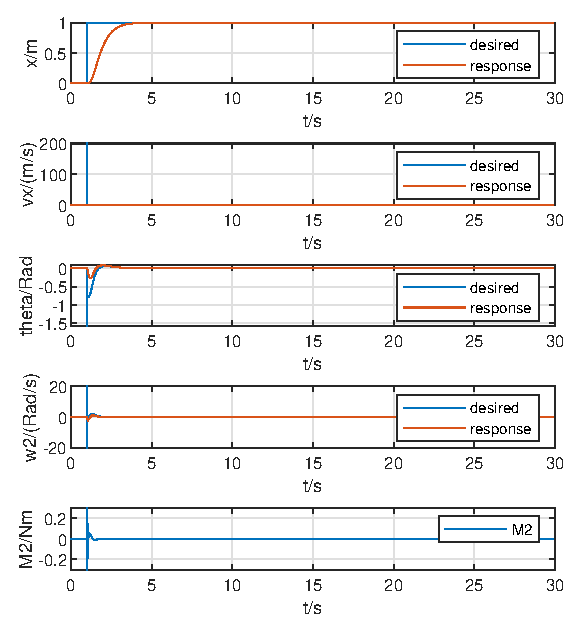
\includegraphics[width=\linewidth]{so3_1.eps}
    \caption{SO(3)}
  \end{subfigure}
  \caption{x轴位置单位阶跃响应对比}
  \label{matlab_阶跃}
\end{figure}

位置的阶跃给速度的期望值带来了微分冲击,这个冲击进一步传导给期望俯仰角,导致期望转矩饱和,PX4在这种情况下出现了震荡。HOFA的扭矩饱和持续时间最小,并且对俯仰角的跟踪也是最好的。三种控制器最终都能无静差地收敛到单位值。表\ref{matlab阶跃对比}定量比较了三种控制器分别使位置到达稳态值$90\%$的上升时间和调整时间($\Delta = 5\%$)。
\begin{table}[!h]
  \centering
  \caption{单位阶跃响应性能对比}
  \begin{tabular}{cccc}
      \toprule
      & HOFA & PID & SO(3) \\
      \midrule
    上升时间 & 1.585s & 1.810s & 1.775s\\
    调整时间($\Delta = 5\%$) & 1.940s & 2.005s &2.145s \\
      \bottomrule
  \end{tabular}
  \label{matlab阶跃对比}
\end{table}
由表\ref{matlab阶跃对比}可知,HOFA的收敛速度要略微优于PID和SO(3)。

\subsection*{单位斜坡输入}

接下来向x轴输入单位斜坡信号,对比x轴位置、速度、角度、角速度和期望扭矩,如图\ref{matlab_t}。
\begin{figure}[!htp]
  \centering
  \begin{subfigure}[t]{0.49\textwidth}
    \centering
    \raisebox{-\height}{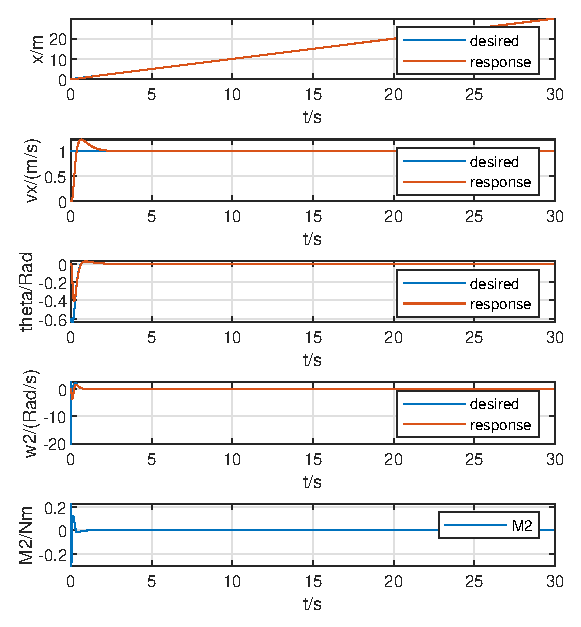
\includegraphics[width=\linewidth]{hofa_t.eps}}
    \caption{HOFA}
  \end{subfigure}\hfill
  \begin{subfigure}[t]{0.49\textwidth}
    \centering
    \raisebox{-\height}{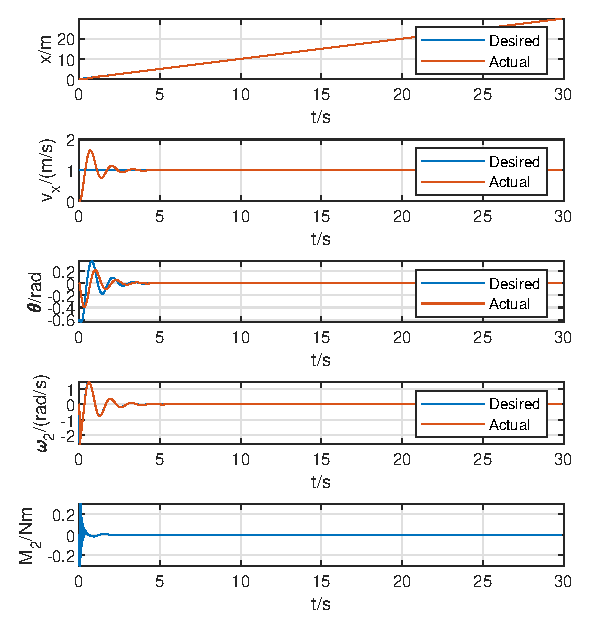
\includegraphics[width=\linewidth]{px4_t.eps}}
    \caption{PID}
  \end{subfigure}\hfill
  \begin{subfigure}[t]{0.49\textwidth}
    \centering
    \raisebox{-\height}{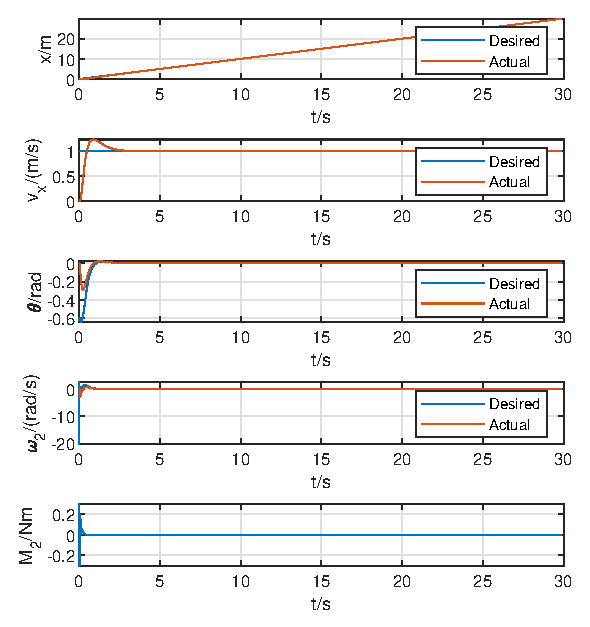
\includegraphics[width=\linewidth]{so3_t.eps}}
    \caption{SO(3)}
  \end{subfigure}
  \caption{x轴位置单位斜坡响应对比}
  \label{matlab_t}
\end{figure}

位置的斜坡输入给速度和姿态角带来了阶跃输入,对于HOFA和SO(3)这两种依赖姿态微分来产生期望角速度的控制器,就使期望角速度和期望力矩饱和,而PID在这一环节只用了比例反馈就相对温和。在匀速飞行阶段,三者的姿态和角速度都保持稳定,这是仿真环境中没有噪声才能做到的。由于位置跟踪的静态误差都是0,因此进一步比较速度曲线,如表\ref{matlab斜坡对比}。三者的速度响应曲线都是欠阻尼,PID的波动更大,当然这可能是参数选择的问题,更快的响应速度意味着更大的超调,反之亦然。HOFA的上升时间小于其他两种控制器,超调量则略微大于SO(3)。调整时间是最优,说明HOFA的非线性前馈补偿项还是给动态过程带来了不小的优化。

\begin{table}[!h]
  \centering
  \caption{单位斜坡响应性能对比}
  \begin{tabular}{cccc}
      \toprule
      & HOFA & PID & SO(3) \\
      \midrule
    位置静态误差                  & 0    & 0 & 0 \\
    速度上升时间                   & 0.37s & 0.385s &0.48s \\
    速度峰值时间                  & 0.66s &0.70s  & 0.90s\\
    速度最大超调量                & $32.0\%$ & $64.7\%$  & $23.7\%$\\
    速度调整时间($\Delta = 5\%$) & 1.67s &2.815s  & 2.09s\\
      \bottomrule
  \end{tabular}
  \label{matlab斜坡对比}
\end{table}
\newpage
\subsection*{“8”字形轨迹综合测试}
  向控制器输入“8”字形轨迹测试控制器的综合性能,得到结果如图\ref{matlab_3d}。可以看出,三种控制方法都能较好地跟上期望轨迹,其中PID仅在开头处的偏差较大,HOFA和SO(3)在三维轨迹图中难以直观分辨性能的高下。
  \begin{figure}[!h]
      \centering
      \begin{subfigure}[t]{0.33\textwidth}
        \centering
        \raisebox{-\height}{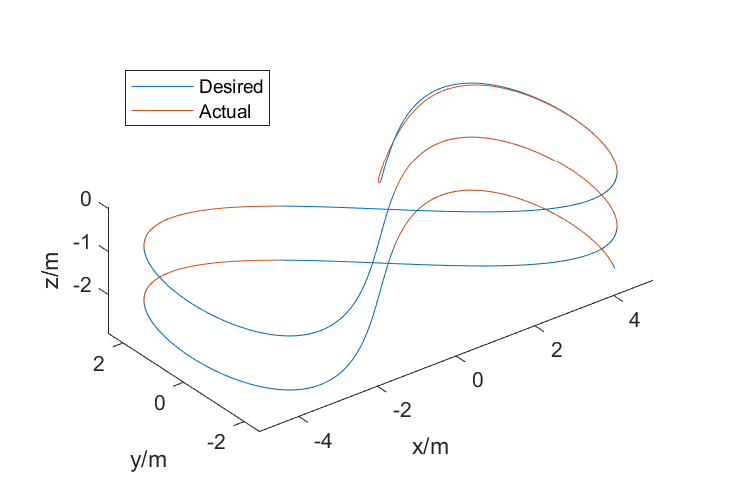
\includegraphics[width=\linewidth]{hofa_3d.eps}}
        \caption{HOFA}
      \end{subfigure}\hfill
      \begin{subfigure}[t]{0.33\textwidth}
        \centering
        \raisebox{-\height}{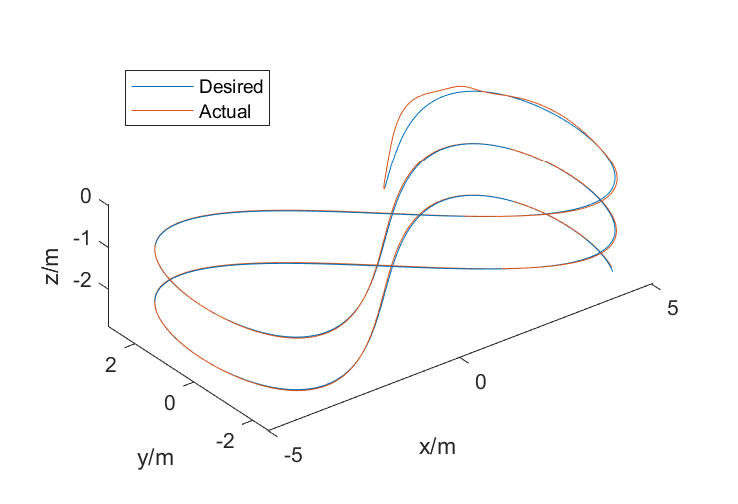
\includegraphics[width=\linewidth]{px4_3d.eps}}
        \caption{PID}
      \end{subfigure}\hfill
      \begin{subfigure}[t]{0.33\textwidth}
        \centering
        \raisebox{-\height}{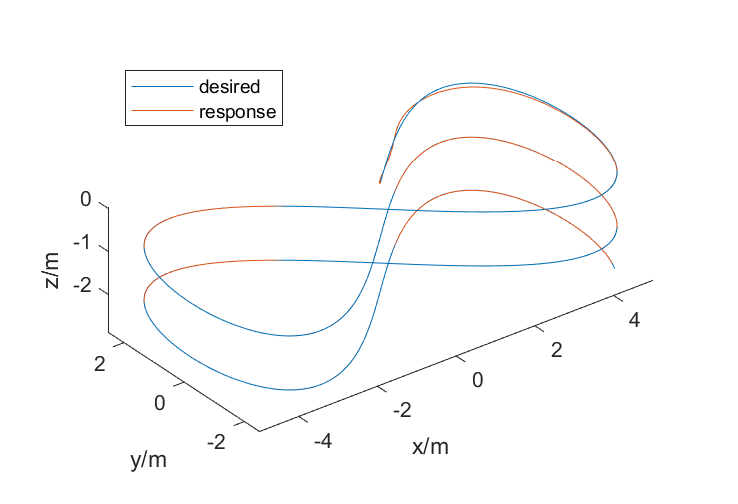
\includegraphics[width=\linewidth]{so3_3d.eps}}
        \caption{SO(3)}
      \end{subfigure}
      \caption{三维轨迹跟踪效果对比}
      \label{matlab_3d}
  \end{figure}
  因此需要进一步看位置和姿态各轴分开的曲线:
  \begin{figure}[!h]
    \centering
    \begin{subfigure}[t]{0.33\textwidth}
      \centering
      \raisebox{-\height}{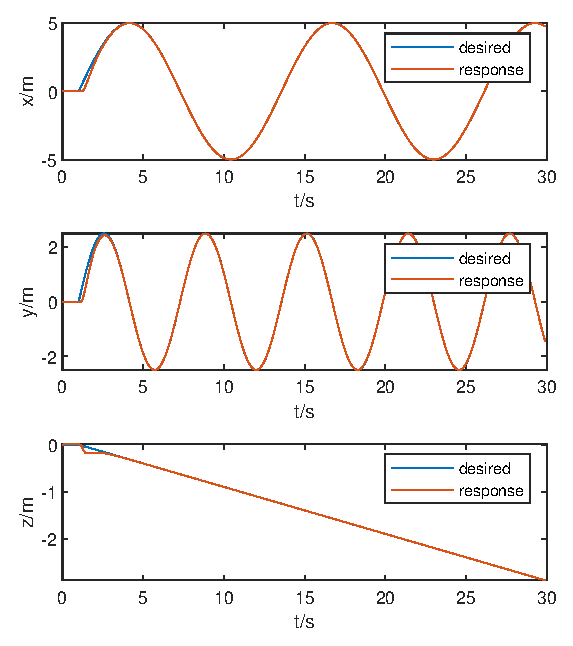
\includegraphics[width=\linewidth]{hofa_x.eps}}
      \caption{HOFA}
    \end{subfigure}\hfill
    \begin{subfigure}[t]{0.33\textwidth}
      \centering
      \raisebox{-\height}{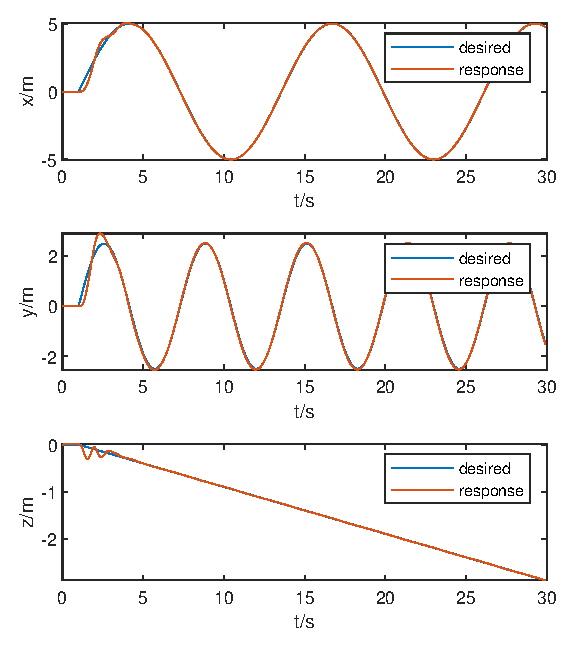
\includegraphics[width=\linewidth]{px4_x.eps}}
      \caption{PID}
    \end{subfigure}\hfill
    \begin{subfigure}[t]{0.33\textwidth}
      \centering
      \raisebox{-\height}{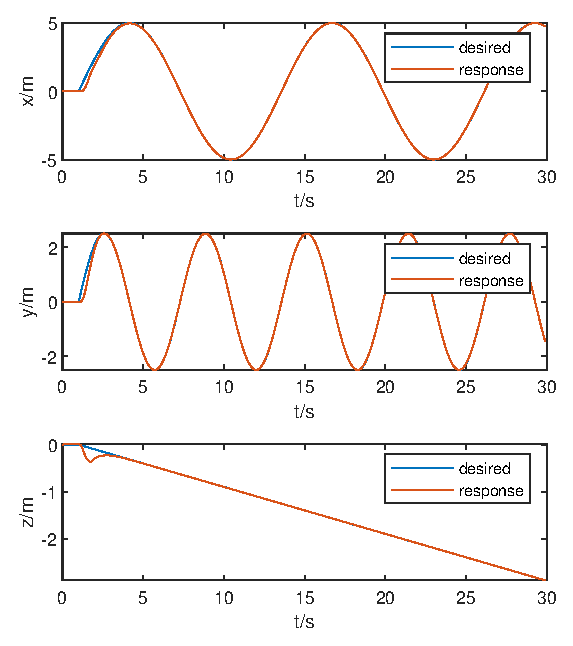
\includegraphics[width=\linewidth]{so3_x.eps}}
      \caption{SO(3)}
    \end{subfigure}
    \caption{三轴位置跟踪效果对比}
    \label{matlab_x}
\end{figure}

\begin{figure}[!h]
  \centering
  \begin{subfigure}[t]{0.33\textwidth}
    \centering
    \raisebox{-\height}{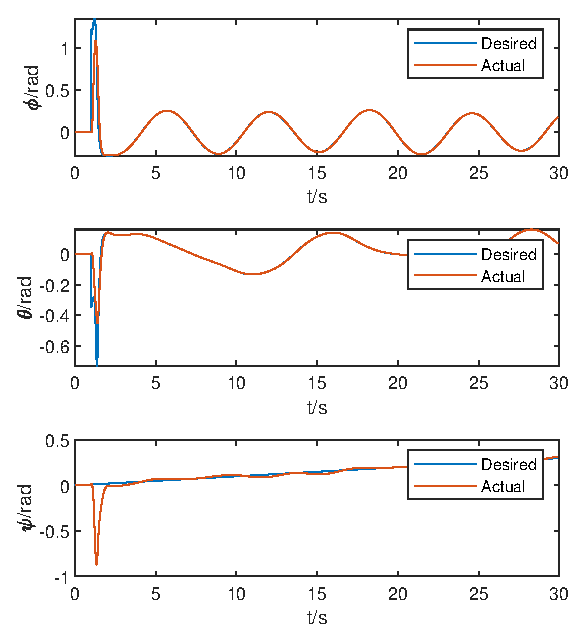
\includegraphics[width=\linewidth]{hofa_angle.eps}}
    \caption{HOFA}
  \end{subfigure}\hfill
  \begin{subfigure}[t]{0.33\textwidth}
    \centering
    \raisebox{-\height}{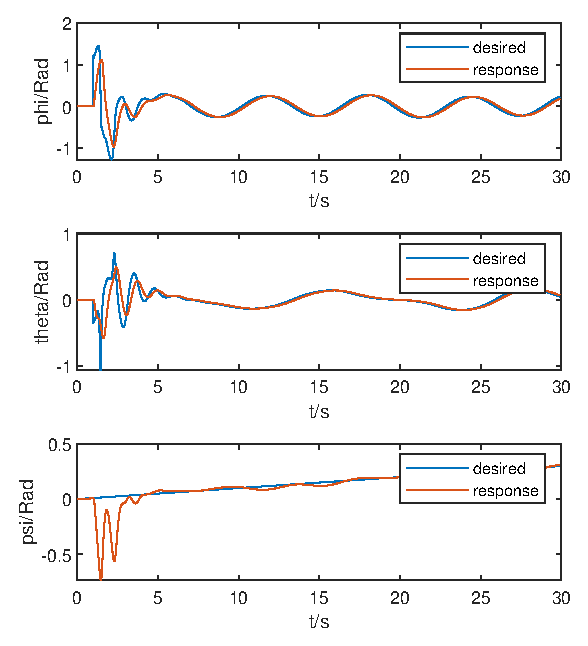
\includegraphics[width=\linewidth]{px4_angle.eps}}
    \caption{PID}
  \end{subfigure}\hfill
  \begin{subfigure}[t]{0.33\textwidth}
    \centering
    \raisebox{-\height}{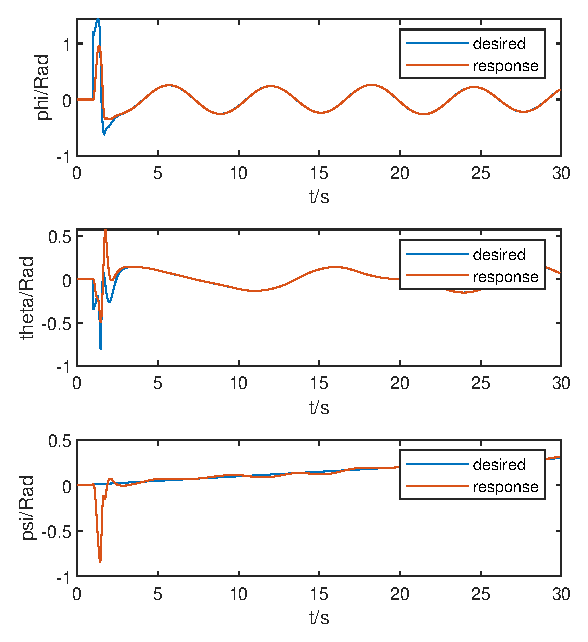
\includegraphics[width=\linewidth]{so3_angle.eps}}
    \caption{SO(3)}
  \end{subfigure}
  \caption{三轴姿态角跟踪效果对比}
  \label{matlab_angle}
\end{figure}

从图\ref{matlab_x},\ref{matlab_angle}中来看,HOFA相较于SO(3)在位置环的优势并不明显,但在姿态环,HOFA的跟踪效果有较为显著的优势。在设定角度超过$50^\circ$的情况下,HOFA仍能做到良好的跟踪,同时保持飞机的稳定飞行。为了定量地对比三者的跟踪性能,引入指标
  $$e_d=\frac{\sum_0^{T}||x-x_d||}{T} ,\quad e_{angle}=\frac{\sum_0^{T}|\phi-\phi_d+\theta-\theta_d+\psi-\psi_d|}{T},$$

  $$J=\sum_0^{T}(p-p_d)^T Q_x(p-p_d)+u^T R_x u \quad p=\begin{bmatrix}
    x \\ v
  \end{bmatrix}.$$
  \begin{table}[!h]
    \centering
    \caption{HOFA方法与对照组的平均误差对比}
    \begin{tabular}{cccc}
        \toprule
        & 平均距离误差:$e_d$ (m)& 平均角度误差:$e_{angle}(Rad)$  & 最优控制指标:$J$ \\
        \midrule
        HOFA & 0.0296 & 0.0051 &49731 \\
        PID & 0.0710 & 0.0628 &54410 \\
        SO(3) &0.0408  &0.0143 &50277 \\
        \bottomrule
    \end{tabular}

    \label{matlab对比}
\end{table}
从表\ref{matlab对比}中可以看到,HOFA相较于PID和SO(3)均有不小的优势,尤其是在姿态控制上,HOFA能做到更高的跟踪精度。

在实践中,执行器的能力存在上限,并且轨迹中的不连续点会引起微分冲击,因此在控制器中需要做限幅处理以避免极端大的控制量对系统造成不良影响。而限幅的具体数值也要根据控制器的输出做调整。从图\ref{matlab_fM}可知,除了在开头的阶跃处,当飞行进入稳定阶段时,期望的力矩非常小,远远不会达到设定的上限。
\begin{figure}[!h]
  \centering
  \begin{subfigure}[t]{0.33\textwidth}
    \centering
    \raisebox{-\height}{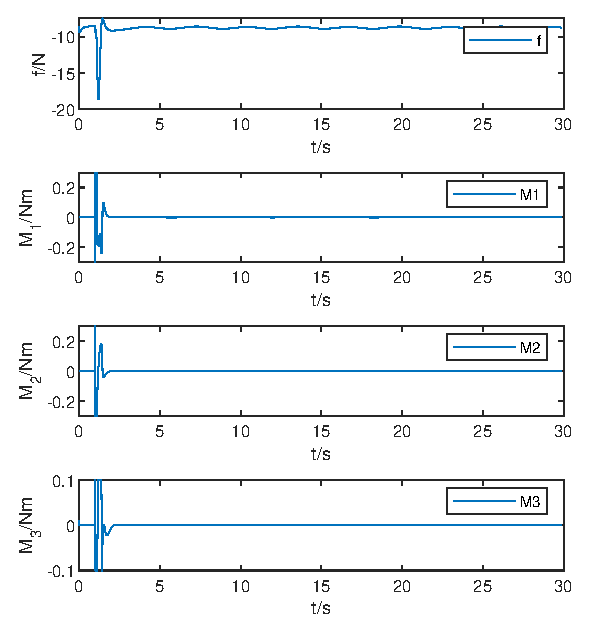
\includegraphics[width=\linewidth]{hofa_fM.eps}}
    \caption{HOFA}
  \end{subfigure}\hfill
  \begin{subfigure}[t]{0.33\textwidth}
    \centering
    \raisebox{-\height}{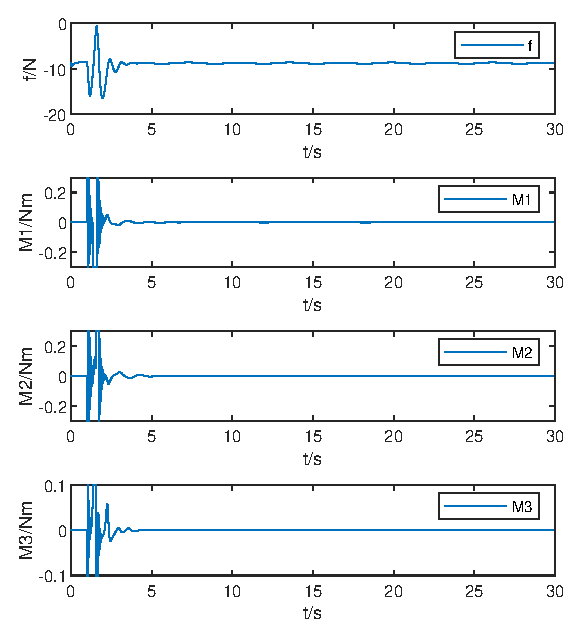
\includegraphics[width=\linewidth]{px4_fM.eps}}
    \caption{PID}
  \end{subfigure}\hfill
  \begin{subfigure}[t]{0.33\textwidth}
    \centering
    \raisebox{-\height}{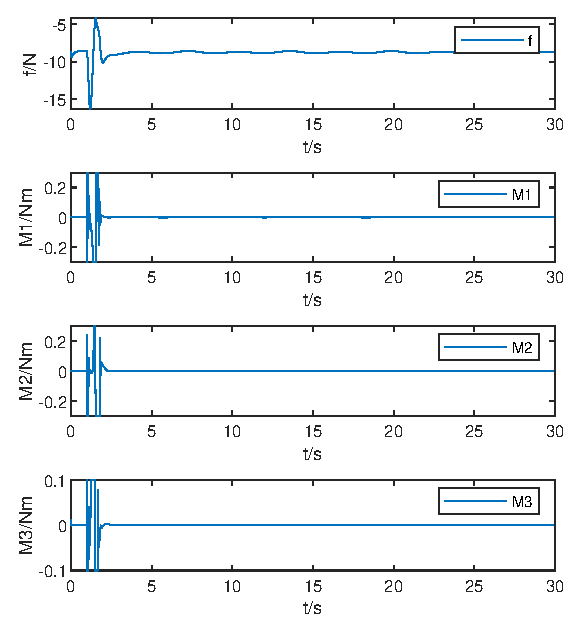
\includegraphics[width=\linewidth]{so3_fM.eps}}
    \caption{SO(3)}
  \end{subfigure}
  \caption{期望拉力与力矩对比}
  \label{matlab_fM}
\end{figure}

% %%
% \begin{figure}[!h]
%   \centering
%   \begin{subfigure}[t]{0.33\textwidth}
%     \centering
%     \raisebox{-\height}{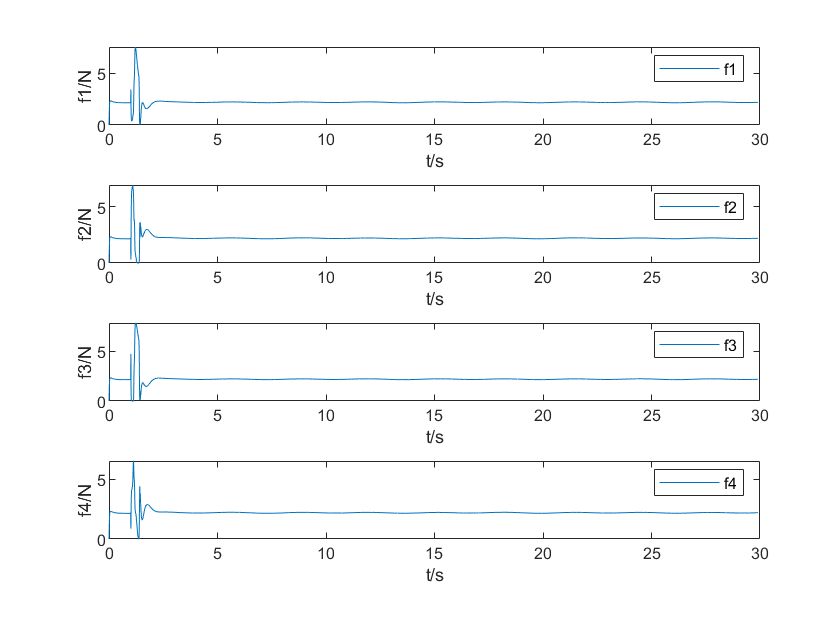
\includegraphics[width=\linewidth]{hofa_f1234.png}}
%   \end{subfigure}\hfill
%   \begin{subfigure}[t]{0.33\textwidth}
%     \centering
%     \raisebox{-\height}{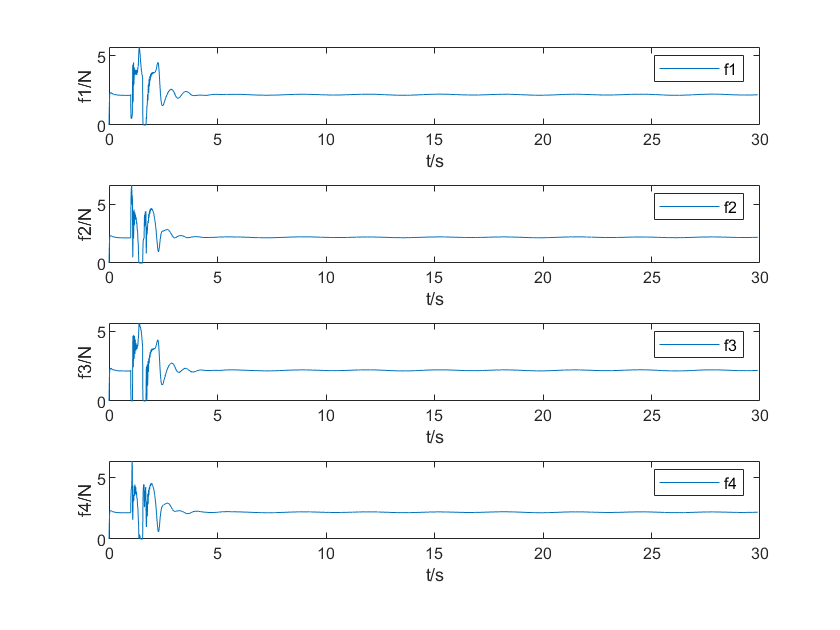
\includegraphics[width=\linewidth]{px4_f1234.png}}
%   \end{subfigure}\hfill
%   \begin{subfigure}[t]{0.33\textwidth}
%     \centering
%     \raisebox{-\height}{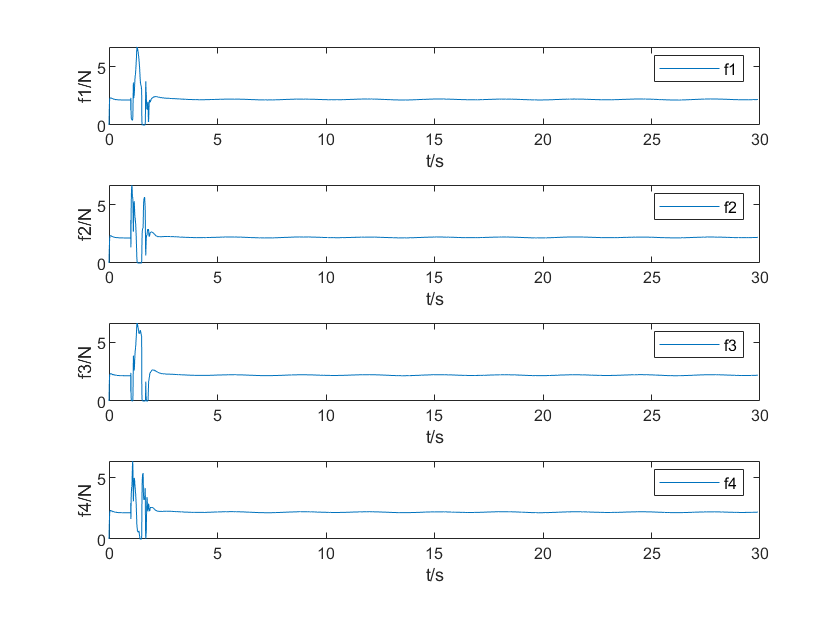
\includegraphics[width=\linewidth]{so3_f1234.png}}
%   \end{subfigure}
%   \caption{电机期望拉力对比:HOFA,PX4,SO(3)}
%   \label{matlab_f1234}
% \end{figure}

% %%

\section{期望力矩组分分析}
在以上数值实验之外,我们还要探究控制器输出的期望力矩的组分,以明确是哪些项在控制中起到了关键作用。姿态环的输出的期望力矩由三部分组成,
$$M=-B^{-1}(R_d,R) A_d(R_d,\omega_d,\dot \omega_d,R,\omega)+\omega \times J\omega +B^{-1}(R_d,R)M^*(R_d,\omega_d,R,\omega),$$
前两项可以视作前馈补偿,第三项可以视作反馈。除$wJw$外,都含有期望角速度,这会在外部输入出现不连续时带来冲击,$A_d$甚至含有期望角加速度,冲击更为剧烈。三部分均含有角速度,Matlab阶段较为理想,但在实机实验中角速度受电机振动影响,很容易出现高频的剧烈抖动,这也会带来不良影响,因此要降低角速度的反馈权重。

Matlab中虽然无法模拟角速度的高频抖动,但是能体现外部位置阶跃输入带来的期望角速度冲击给期望力矩计算带来的影响,如图\ref{fig:com}所示。在位置阶跃输入时,确实给$A_d$和$M^*$部分带来了冲击。在角速度很小的情况下,第二部分的数值几乎可以忽略。在大部分情况下,反馈项和整体的趋势相同,或者说反馈项主导了整体的走势。$A_d$和整体的吻合程度略低一些,$wJw$的走势则几乎与整体无关。
\begin{figure}[!h]
  \centering
  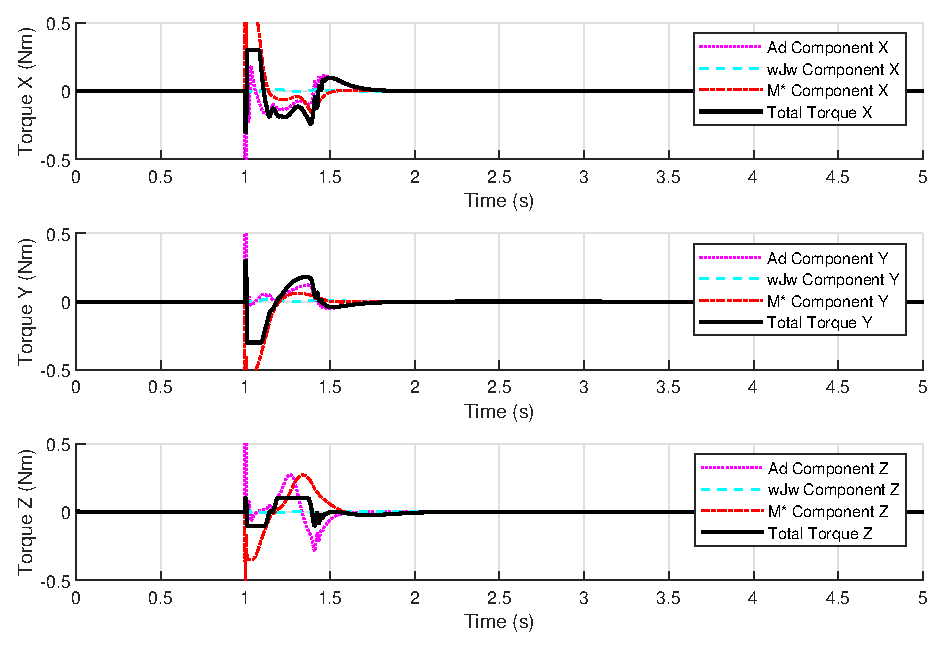
\includegraphics[width=0.9\textwidth]{component.eps}
  \caption{姿态环输出期望力矩组成}
  \label{fig:com}
\end{figure}
\newpage
\section{本章小结}
本章在深入探讨了几种主流姿态表示方式的优劣势后,选择了基于旋转矩阵的姿态表示来建立四旋翼的动力学模型。明确了机身坐标系和世界坐标系的定义,推导了四旋翼的刚体动力学模型。然后,在动力学模型的基础上,将欠驱动的四旋翼分解成姿态环路和位置环路,对具有全驱特性的姿态环路应用高阶全驱系统理论,使其从非线性系统转化为线性系统,随即应用LQR控制。接着,在Matlab中展开数值仿真,将HOFA与经典的控制方法对比并根据实验数据展开分析。在单位阶跃和单位斜坡信号的输入下,HOFA具有更快的收敛速度和追踪性能。在“8”字型轨迹的综合测试下,HOFA具有更高的跟踪精度,并且在优化指标上,验证了LQR的最优性能。总而言之,在较为接近理想化模型的Matlab仿真中,HOFA展现出了相较于PID和SO(3)两种经典控制方法的优势。最后,分析了控制器输出的期望力矩的组分,明确了反馈项才是输出的主导组分。